%!TEX root = ../dokumentation.tex

%TODO: Einleitungen überarbeiten
\chapter{Konzept}\label{cha:Konzept}
\section{Anforderungen}\label{sec:Anforderungen}
Im Folgenden werden die Funktionalitäten erläutert, die die Anwendung besitzen soll. Hauptziel ist es, dass Nutzer, parallel zur Nutzung des Chats, ein 4-gewinnt-Spiel spielen können. Dabei spielen jeweils zwei Spieler gegeneinander, wobei die Anwendung von mehr als zwei Nutzern gleichzeitig genutzt werden können soll. Vor der Teilnahme an dem Chat und einem Spiel sollen sich die Nutzer einloggen. Dafür soll eine Registrierungsmöglichkeit geschaffen werden und die Registrierungsdaten sollen in einer Datenbank gespeichert werden. Wenn ein Spieler ein Spiel starten möchte, so soll dieser mit dem nächsten Spieler spielen können, der auch ein Spiel starten möchte.
\section{Übersicht}\label{sec:Übersicht}
Die Anwendung besteht aus zwei verschiedenen Teilen, die beide mittels Docker deployt werden. 
Der eine Teil beinhaltet die Chat-Anwendung und die Spiellogik, der andere beinhaltet eine MongoDB, welche zum Speichern der Benutzer-Login-Informationen verwendet wird.\\
Abbildung \ref{fig:koncept} beinhaltet eine Übersicht über die Komponenten der Anwendung.

\begin{figure}[H]
\centering
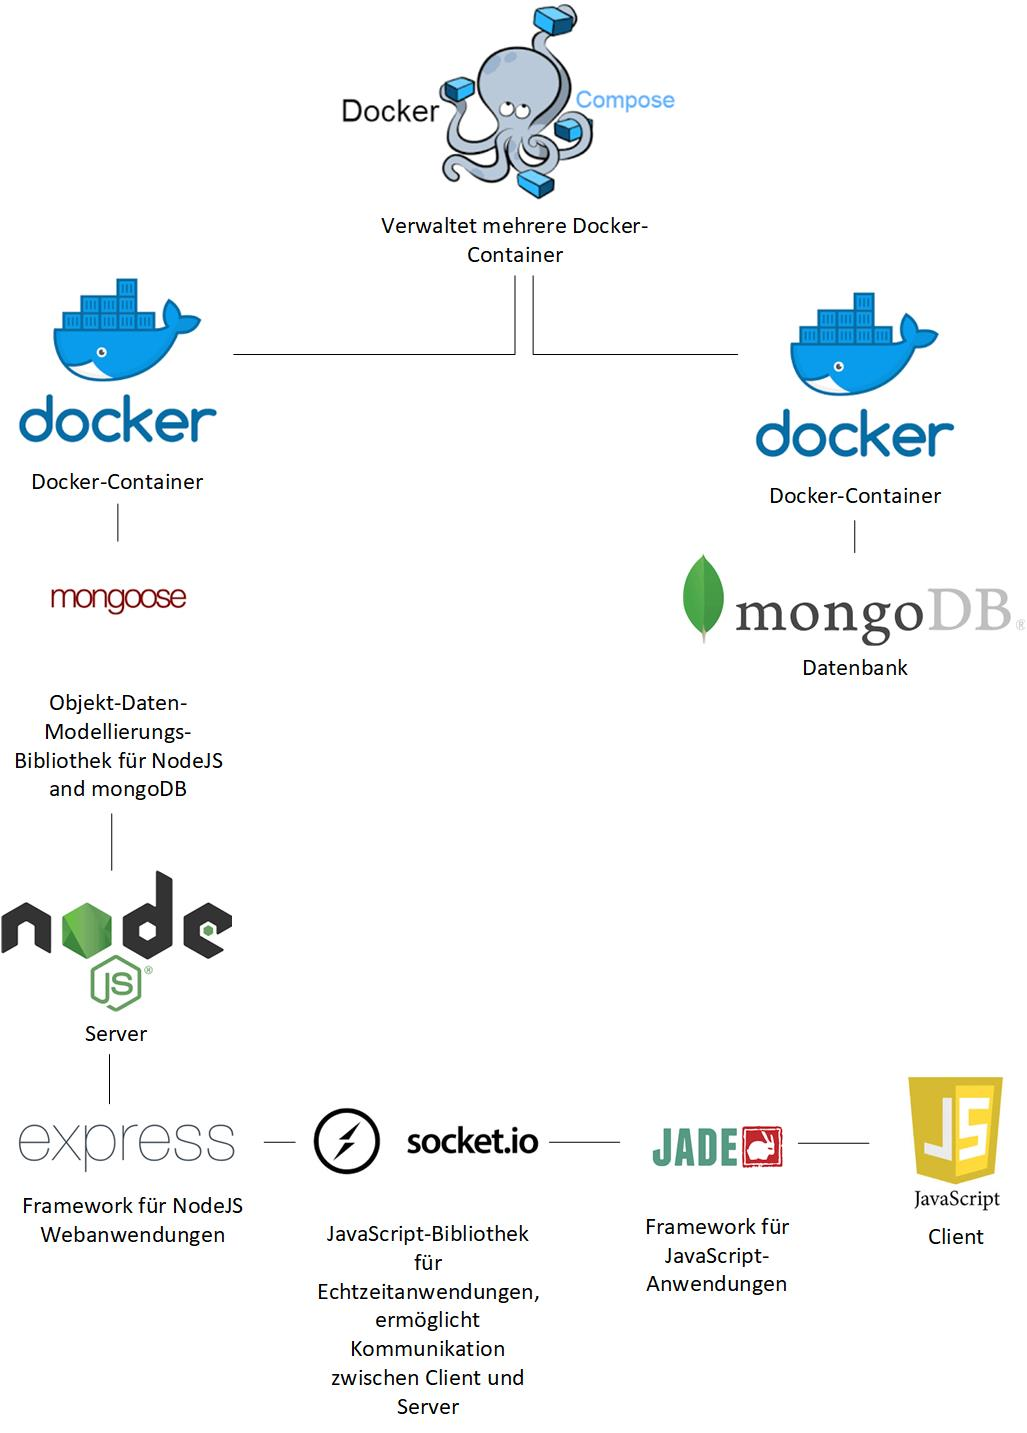
\includegraphics[width=1\textwidth]{images/uebersicht.jpg}
\caption{Übersicht der Anwendung}
\label{fig:koncept}
\end{figure}


\section{Login und Registrierung}\label{sec:Login}
Beim Login hat der User die Möglichkeit, sich zu registrieren oder sich direkt einzuloggen. Die Login-Informationen werden bei der Registrierung in der MongoDB gespeichert und verwaltet. 

\section{Spiel}\label{sec:Spiel}
Nachdem zwei Spieler ein Spiel begonnen haben, können sie gegeneinander spielen. Mittels Buttons kann ausgewählt werden, in welche Reihe sie setzen möchten. Hierbei muss überprüft werden, ob der Spieler an der Reihe ist und ob die Reihe, in der der Stein gesetzt werden soll, nicht voll ist. Außerdem muss geprüft werden, ob es ein Spieler geschafft hat, vier Steine in eine vertikale, horizontale oder diagonale Reihe zu platzieren. Nachdem das Spiel entweder gewonnen oder unentschieden beendet wird, wird das aktuelle Spielfeld deaktiviert und es besteht die Möglichkeit, ein neues Spiel zu starten. Um dem Spieler Informationen über den Spielstand mitzuteilen, schickt ein sogenannter Gamemaster Nachrichten an die Spieler.  Diese Nachrichten werden wie die Chat-Nachrichten über den Websocket geschickt.

Das Spielfeld besteht jeweils aus 7 Spalten und 6 Zeilen, dieses wird als zweidimensionales Array gespeichert. Wenn ein Element den Wert Null hat, bedeutet das, dass kein Spieler an dieser Position einen Stein gesetzt hat.
\section{Nachrichtenfilterung}\label{sec:Nachrichtenfilter}
Typischerweise werden bei einer Websocket-Anwendung allen Usern die eintreffenden Nachrichten angezeigt. Um dies zu umgehen und nur den am Spiel beteiligten Spielern relevante Nachrichten anzuzeigen, enthält die Nachricht die Namen der beiden am Spiel beteiligten Parteien. So kann der Client ermitteln, ob er am Spiel beteiligt ist und aufgrund dessen die Nachrichten anzeigen oder ignorieren. 

\section{Gleichzeitiges Spielen mehrerer Spieler}\label{sec:Multiplegames}
Um es mehr als zwei Spielern zu ermöglichen, gleichzeitig zu spielen, wird ein zweidimensionales Array genutzt. In einer Dimension sind jeweils ein Spielbrett, die zwei Spieler und der Spieler, der aktuell an der Reihe ist, gespeichert. In der anderen Dimension werden die verschiedenen Spiele gespeichert. Sobald ein Spiel beendet wird, werden die zugehörigen Variablen aus dem Array mit dem Wert null belegt. Wenn ein neues Spiel begonnen wird, wird durch das Array iteriert und die erste freie Position verwendet, um dieses Spiel zu speichern. 
